\documentclass[10pt]{article}
\usepackage[T1]{fontenc}
\usepackage{lmodern,amsmath,amssymb,graphicx,hyperref,array}
\usepackage[margin=.75in]{geometry}
\setlength{\parindent}{0pt}\setlength{\parskip}{6pt}
\begin{document}
\begin{center}
{\Large Actual all-node moments and whole-chart precision}\\[4pt]
14 November 2026; 38 authored Lean statements\\
Source \texttt{3299b929faad599061b1c13eed9de02ef7e806f2}
\end{center}
\textbf{Construction.} For the same completed auxiliary orientation polynomial,
the new component constructs first-jet moment factors at every retained
nonzero source node, then derives a finite geometric approximation for every
coefficient of its actual crossing chart. The approximation is per entry;
compact whole-polynomial matrix factors are a separate open obligation.
All records are unsigned [pcc:unverified].

\textbf{Actual inputs.} Let $L=2^a$, $S=\{-L,\ldots,L-1\}\subset\mathbb Q$,
$t\in S\cap\mathbb Z$ nonzero with $v_2(t)=i<u\le a$, and actual ports
$x,y<L$ with equal bit $i$. Use natural multiplicities $m_j$, the same
completed $W_{xy}(T)$, and
\[
 r=x\bmod2^u,\quad h=x\mathbin{\mathrm{div}}2^u,\quad
 \delta_x=y-x,\quad\delta_r=y-r,\quad\alpha=2^{a+1}.
\]
The reference $c$ is the existing nonzero diagonal first jet at the negative
pole $-2^i$, with valuation $w=a+1-i+G_i$, where
$G_i=m_i-\sum_{j<u}(j-i)_+m_j$. It is not the potentially zero local
first jet at $t$. Define $P_x(Z)=W_{xy}(t+\alpha Z)/c$ and $P_r$ similarly.
The previous all-node source derives $P_x(0)=0$ and normalized coefficient
$n+1$ of weight at least $n$, hence integral whole polynomials
[pcc:unverified].

\textbf{First-jet moments.} Literal prototype denominators give even slopes
\[
 e_t=\frac{2^u}{t-\delta_r},\qquad e_j=\frac{2^u}{2^j-\delta_r},\qquad
 D_H(H)=(1+e_tH)\prod_{j\in M_{xy}}(1+e_jH)^{m_j}.
\]
Its constant is one and coefficient $b$ has valuation at least $b$.
The actual normalized first-jet family is its prototype first jet times
$D_H(h)^{-1}$. Standard inverse-series truncation below $k$ yields constructed
$2^u k$ factors, left weight $b$, integral right, and normalized residual
$k$. Actual $c$ scaling gives left weight $w+b$ and residual $w+k$.
No positive-multiplicity or nonzero local-jet assumption enters this profile
[pcc:unverified].

At a positive retained anchor with $m_i>0$, every actual first crossing jet
and corresponding right moment factor is zero. This control concerns the first jet only [pcc:unverified].

\newpage
\begin{center}{\Large Actual polynomial denominator and geometric error}\end{center}
\textbf{Derive the identity from $W$.} Exact retained-mask comparison and
the original nodal puncture identity give
\[
 (T-\delta_x)W_{xy}(T)=q(T-\delta_r)W_{ry}(T),\qquad
 q=\prod_{j\in M_{xy}}
       \left(\frac{2^j-\delta_r}{2^j-\delta_x}\right)^{m_j}.
\]
Only actual nonzero denominators are inverted. No local first jet is cancelled.
Put $d_x=t-\delta_x$, $d_r=t-\delta_r$ and $\lambda=\alpha/d_r$. Construct
\[
 D(Z)=q^{-1}\left(\frac{d_x}{d_r}+\lambda Z\right),\qquad
 N(Z)=(1+\lambda Z)P_r(Z).
\]
The literal row identity proves $D P_x=N$. Actual crossing-bit denominators
give $q^{-1}\equiv d_x/d_r\equiv1\pmod2$ and $v_2(\lambda)\ge1$.
Thus $D-1$ has content at least one and $P_x,N$ are integral. These facts
are proved for the actual inputs, not supplied as favorable premises
[pcc:unverified].

\textbf{Finite construction.} Define
\[
 S_k(D)=\sum_{n=0}^{k-1}(1-D)^n,\qquad A_{x,k}=N S_k(D).
\]
The finite geometric identity is $D S_k=1-(1-D)^k$. If $D-1$ has content
one, multiplication by $D$ preserves a desired finite content bound on an
integral polynomial: starting at content zero, repeatedly write
$R=DR-(D-1)R$ to increase the bound to $k$.
This yields
\[
 \operatorname{Content}_k(P_x-A_{x,k}),\qquad
 \operatorname{Content}_{w+k}
   \bigl(W_{xy}(t+\alpha Z)-cA_{x,k}(Z)\bigr).
\]
Here content means the bound holds for every polynomial coefficient,
including all higher chart coefficients. It permits a vanishing local
first jet and uses no inverse of it [pcc:unverified].

\textbf{Degree accounting.} The actual $D$ is affine in $Z$.
For $k>0$, the proof bounds $\operatorname{natdeg} S_k\le k-1$, and
\[
 \operatorname{natdeg}A_{x,k}\le\operatorname{natdeg}P_r+k.
\]
The $k=0$ approximation is zero and is handled separately. This bounds
polynomial degree, not coefficient bit sizes, construction time or storage
[pcc:unverified].

\newpage
\begin{center}{\Large Two constructions and the compact-factor gap}\end{center}
\begin{center}
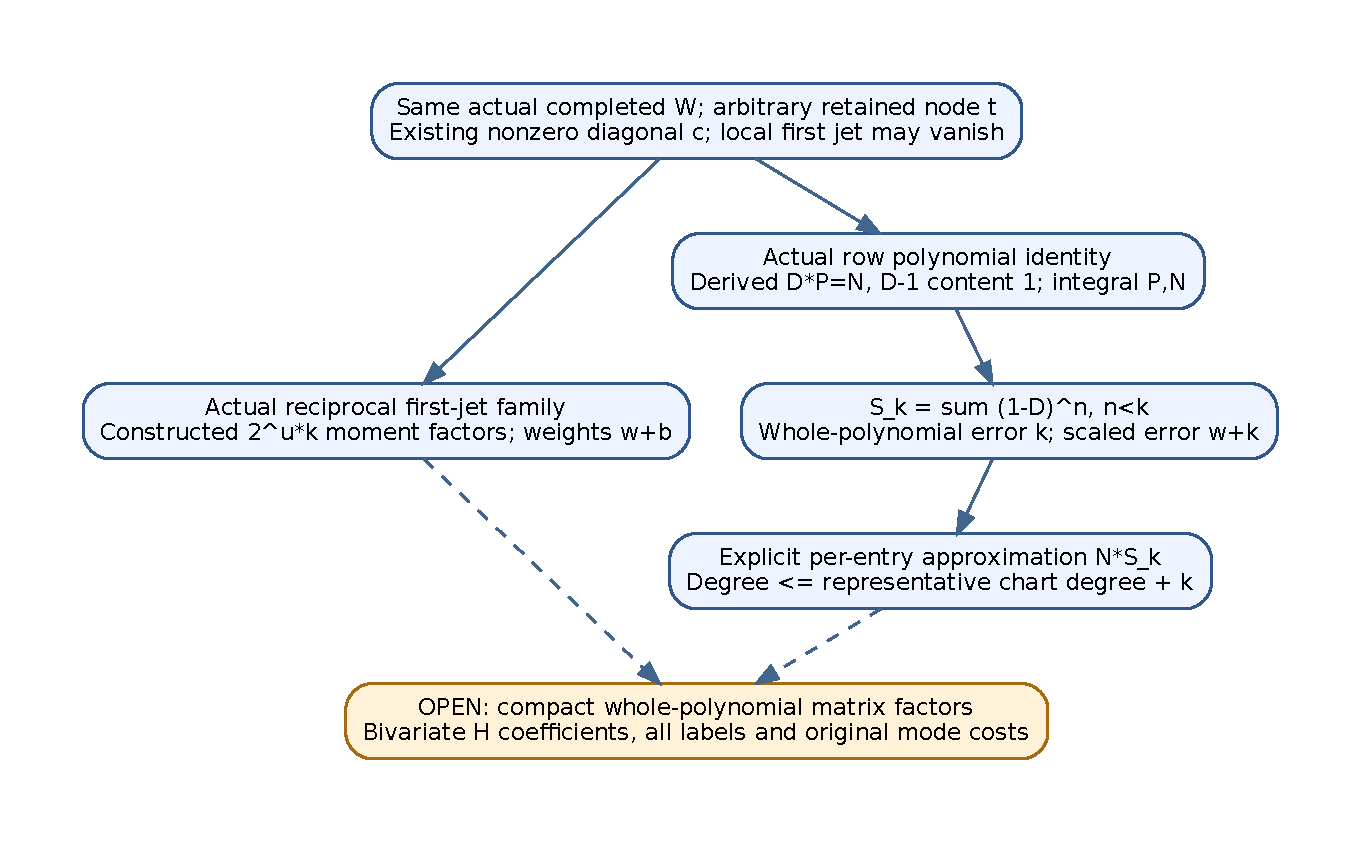
\includegraphics[width=.97\linewidth,height=4.1in,keepaspectratio]{dependencies.pdf}
\end{center}
The $2^u k$ matrix factors concern the \emph{first jet}. The full-polynomial
approximation $A_{x,k}$ still depends on the individual row through $q$ and
$d_x$. No compact full-polynomial matrix factorization is claimed by this
component [pcc:unverified].

\textbf{Next discriminating construction.} Write the actual row quotient as
$H$, construct the polynomial denominator
\[
 \mathcal D(H,Z)=(1+e_tH+\lambda Z)
       \prod_{j\in M_{ry}}(1+e_jH)^{m_j},
\]
and its finite geometric approximation. Prove coefficient-$H^b$ content
at least $b$, then truncate $b\ge k$ with an actual error bound at integer
$h$. This is a prospective route to compact whole-polynomial factors; its
coefficient bridge and matrix product are not part of these 38 statements
[pcc:unverified].

Every residue/moment label must be charged. The original primary interface
allows at most $6M/D_i$ modes per weight, $D_i=L/2^i$; a $2^u$ inventory
can exceed its old $2^{i+1}$ tile count. Full coefficient construction,
entry and bit costs, degree, precision, recovery, recursion, public relations,
finder, field and scalar extraction, retries and expected cost remain
explicit obligations.

\newpage
\begin{center}{\Large Source bindings, validation and preserved failures}\end{center}
The new isolated project builds all 38 authored statements without warnings.
The pinned shared gate audits 39 declarations, zero extra trusted axioms,
exit 0. Import-inclusive fresh replay is running, not passed. Six central printed dependencies
contain only \texttt{propext}, \texttt{Classical.choice}, \texttt{Quot.sound}.
All source records are unsigned [pcc:unverified].

\begin{center}\small
\begin{tabular}{p{.64\linewidth}p{.25\linewidth}}
\texttt{actual\_node\_moment\_profile}&PCC-20261114-ae019d\\
\texttt{actual\_row\_denominator\_identity}&PCC-20261114-b2de93\\
\texttt{actual\_whole\_chart\_precision}&PCC-20261114-1802a0\\
\texttt{actual\_weighted\_whole\_chart\_precision}&PCC-20261114-96a569\\
\texttt{actual\_approximation\_degree}&PCC-20261114-7649ed
\end{tabular}
\end{center}
Full statements govern their hypotheses. Statement bindings, source pins
and the prospective contract are in
\begin{center}\small
\path{../evidence/claim-pins.json}\\
\path{../evidence/source-freeze.json}\\
\path{../PROTOCOL.md}.
\end{center}
Gate data is PCC-20261114-03eb52. Local draft007 data is PCC-20261114-496991;
that observation alone is not independent gate/replay coverage
[pcc:unverified].

\textbf{Reproducibility.} Lean4.35.0, CryptoLean and Mathlib revisions:
\begin{center}\small
\texttt{148f5dc389b341401e06d76abe7783c4ccf42f2e}\\
\texttt{cfc55fc58714a59dc06e6e79edc6d1d95140d3c2}.
\end{center}
The source is an exact copy of accepted draft007. All earlier failed sources,
eight build logs/exits and local data receipts remain under
\path{../../nodes/moment-evidence/}. Failures include private-import visibility,
wrong Lake working directory, an unreduced class port, a deprecated API,
and two exact argument/wrapper mismatches. No linter was disabled or desired
content/factor witness added.

\textbf{Sources checked.} KB unavailable as journaled. Read exact parent
Node/Moment/Content/Anchor denominator, inverse-series, graded entry and
row-polynomial proofs; pinned Mathlib geometric-sum and polynomial-degree
APIs; earlier primary D.4.3--7 and contraction precision/cost reviews.
Standard finite geometric sums and inverse-series moments are reused without
a novelty, priority, fastest-method or measured speed assertion.

No native crypto, attack, F4/msolve, timing, scaling, paid or cloud experiment
ran. The original norm fixture remains unlaunched under its unchanged
checkpoint transport blocker. No measured result updates canonical IC
graphs/leaderboards; the diagram records proof dependencies.

The parent arbitrary-node42/44/fresh0 project and all90 artifact pins remain
exact, as do earlier parent checkpoints. The protected concurrent PCC
histories remain unresolved; auto-merge stays off. No claim rewrite,
rechain, side selection, signature, prefix waiver or force push is attempted.
\end{document}
